\documentclass[12pt, a4paper]{article}

\usepackage[utf8]{inputenc}
\usepackage[T1]{fontenc}
\usepackage{graphicx}
\usepackage{geometry}
\geometry{margin=2.5cm}
\usepackage{parskip}
\usepackage{url}
\usepackage{tikz}
\usetikzlibrary{positioning, arrows.meta, decorations.pathreplacing, fit}
\usepackage[export]{adjustbox}
\usepackage{minted}
\usepackage{caption}
\captionsetup{font=small, labelfont=bf, skip=10pt, aboveskip=10pt, margin=2em}

\begin{document}

\begin{titlepage}
  \centering
  \vspace*{1cm}
  \includegraphics[width=0.35\textwidth]{images/hbku.png}\\[2cm]
  {\LARGE\bfseries Wireless Keyboard System Using NRF24L01 Radio Communication Between STC89C52RC and ESP32\par}
  \vspace{1.5cm}
  {\large Marwan Humaid \hspace{2em} Rama Hamze\par}
  \vspace{1cm}
  {\normalsize Instructor: Dr.\ Bo Wang\par}
  \vspace{1cm}
  {\normalsize CPEG 300: Embedded System Design\par}
  \vfill
  {\normalsize March 24, 2026\par}
  \vspace{1cm}
\end{titlepage}

\begin{abstract}
This report demonstrates wireless communication using the NRF24L01 2.4\,GHz radio transceiver to link two heterogeneous microcontrollers: an ESP32-DevKitC~V4 and an STC89C52RC (8051 architecture). The demonstration takes the form of a wireless keyboard, where keystrokes typed on a PC are transmitted over the radio link and displayed in real time on a 16$\times$2 LCD connected to the STC89C52RC. Since the NRF24L01 cannot connect directly to a PC, an ESP32 serves as a USB-to-radio bridge, driving its NRF24L01 via hardware SPI, while the STC89C52RC communicates with its NRF24L01 through a bit-banged SPI implementation. The report covers the radio link bring-up process, including initialization timing workarounds for the NRF24L01 on the 8051, reliability challenges faced during development (clone module quirks, a faulty transceiver with a non-functional RF front-end but working SPI), and statistics from stress testing the final implementation, which achieves 100\% packet delivery across sustained 1000-packet tests using an application-level acknowledgement protocol.
\end{abstract}

\section{Introduction}

The STC89C52RC~\cite{stc89c52} (hereafter \textbf{STC}) is an 8-bit microcontroller based on the Intel MCS-51 (8051) architecture, a design dating back to the early 1980s. While it remains commonly used in embedded systems coursework, its age brings significant hardware constraints that complicate modern peripheral integration. In this project, the STC89C52RC is mounted on a \textbf{Prechin C51 development board}, which integrates a CH340G USB-to-UART converter for serial communication and includes a dedicated socket for the NRF24L01~\cite{nrf24l01} (hereafter \textbf{NRF}) radio module. However, the Prechin board routes many of the chip's I/O pins to on-board peripherals (LEDs, buzzers, stepper motor drivers, etc.), creating \textbf{port multi-connection} conflicts. Since the pin assignments are fixed by the board layout (NRF on P1, LCD1602 data on P0 with control lines on P2, UART on P3), any additional component must avoid conflicting with what is already wired. This constrains the project: the LCD, radio, and serial debugging must coexist on ports that are also shared with on-board LEDs, buzzers, and other peripherals. The STC also lacks hardware SPI, so all radio communication must be bit-banged in software, a process that is slower and more sensitive to timing than a dedicated peripheral.

The goal of this project is to demonstrate \textbf{wireless communication} using the NRF radio transceiver between the ESP and the STC. As a concrete application of this radio link, the project implements a wireless keystroke system: the user types on a PC, and the typed characters are transmitted over the 2.4\,GHz link and displayed in real time on a 16$\times$2 LCD connected to the STC.

Since the NRF is a standalone radio transceiver with an SPI interface, it cannot be connected directly to a PC. A second microcontroller, the \textbf{ESP32-DevKitC~V4}~\cite{esp32} (hereafter \textbf{ESP}), is therefore introduced as a USB-to-radio bridge: it connects to the PC over USB serial and drives one NRF module via hardware SPI. A second NRF module is connected to the STC via bit-banged SPI. The ESP receives keystrokes from the PC and forwards them as radio packets; the STC receives these packets and displays the characters on the LCD. This architecture keeps the PC-facing serial interface on the ESP, which has native USB support, while the STC focuses solely on receiving packets and driving the display.

\section{Setup}

The development environment required toolchains for two different architectures (the ESP and the STC) as well as a flashing workflow for each. A key design decision was to make the entire build, flash, and test pipeline operable from the command line. This allowed the use of Claude Code, an AI coding assistant, not only for writing firmware but also for compiling, flashing, running, and reading serial output, all within a single CLI session.

For the ESP, the project uses PlatformIO with the Arduino framework. PlatformIO manages the Espressif~32 toolchain and the RF24 library dependency (v1.4.10) automatically. Building and flashing is a single command: \texttt{pio run -t upload -{}-upload-port COMxx}. The active firmware is selected by copying the desired source file into \texttt{src/main.cpp} before building, since PlatformIO compiles all \texttt{.cpp} files in the \texttt{src/} directory.

For the STC, the Keil $\mu$Vision~5 C51 toolchain is used. The evaluation version imposes a 2\,048-byte code size limit, which constrains the firmware: diagnostic or debugging code must be removed before the final build to stay within budget. Keil can be driven from the command line with \texttt{UV4.exe -j0 -r STC89C52.uvproj}, where \texttt{-j0} suppresses the GUI. Once compiled, the resulting hex file is flashed to the board using \texttt{stcgal}~\cite{stcgal}, an open-source ISP programmer for STC microcontrollers. The STC-ISP protocol requires a power-cycle to enter the bootloader. \texttt{stcgal} automates this by toggling the CH340G serial adapter's DTR pin, but its default DTR polarity is inverted relative to the Prechin board's circuit. A custom patch script (\texttt{patch\_stcgal.py}) corrects this by inverting the assertion logic. With the patch applied, flashing proceeds with \texttt{stcgal -P stc89 -p COMxx -a STC89C52.hex}, followed by a manual power cycle so the NRF gets a clean reset.

The complete build-and-run pipeline for the wireless keyboard is: (1)~build and flash the ESP with the keyboard forwarder firmware via PlatformIO; (2)~build the STC firmware in Keil and flash it via \texttt{stcgal}; (3)~power-cycle the STC board; (4)~run the Python keyboard client, which connects to the ESP's serial port and begins forwarding keystrokes. Characters can be typed manually by the user or written to the serial port programmatically by Claude Code.

\section{Experiments}

The system was developed and validated through a series of incremental experiments, each building on the results of the previous one.

The first step was to verify that the ESP could reliably receive characters from the PC over its USB serial link. A simple Python script using \texttt{msvcrt.getch()} captured individual keystrokes on Windows and forwarded them to the ESP at 115\,200\,baud. The ESP firmware echoed received bytes back to the serial monitor, confirming that the serial path worked end to end before any radio hardware was involved.

With serial confirmed, two ESP boards were each connected to an NRF breakout circuit (Figure~\ref{fig:esp32-nrf}) to test radio communication in isolation. The transmitter (\texttt{tx.cpp}) sent a 32-byte packet every second containing a 16-bit counter and a \texttt{0xAA}/\texttt{0x55} marker pattern. The receiver (\texttt{rx.cpp}) printed incoming packets as a hex dump over serial and toggled an LED on each reception. Both boards used the RF24 Arduino library~\cite{rf24lib} over hardware SPI (VSPI). Radio parameters were set to channel~108, 1\,Mbps data rate, 2-byte CRC, no auto-acknowledgement, and a fixed 32-byte payload. Communication was confirmed in both directions by swapping TX/RX roles. Table~\ref{tab:nrf-pins} lists the NRF pin connections for both boards.

\begin{table}[ht]
\centering
\caption{NRF pin connections on the ESP and STC boards.}
\label{tab:nrf-pins}
\begin{tabular}{lll}
\hline
NRF Pin & ESP (hardware SPI) & STC (bit-banged SPI) \\
\hline
VCC  & 3.3\,V            & 3.3\,V \\
GND  & GND                & GND \\
CE   & GPIO\,4            & P1.2 \\
CSN  & GPIO\,5            & P1.3 \\
SCK  & GPIO\,18           & P1.7 \\
MOSI & GPIO\,23           & P1.1 \\
MISO & GPIO\,19           & P1.6 \\
IRQ  & N/C                & N/C \\
\hline
\end{tabular}
\end{table}

\begin{figure}[ht]
\centering
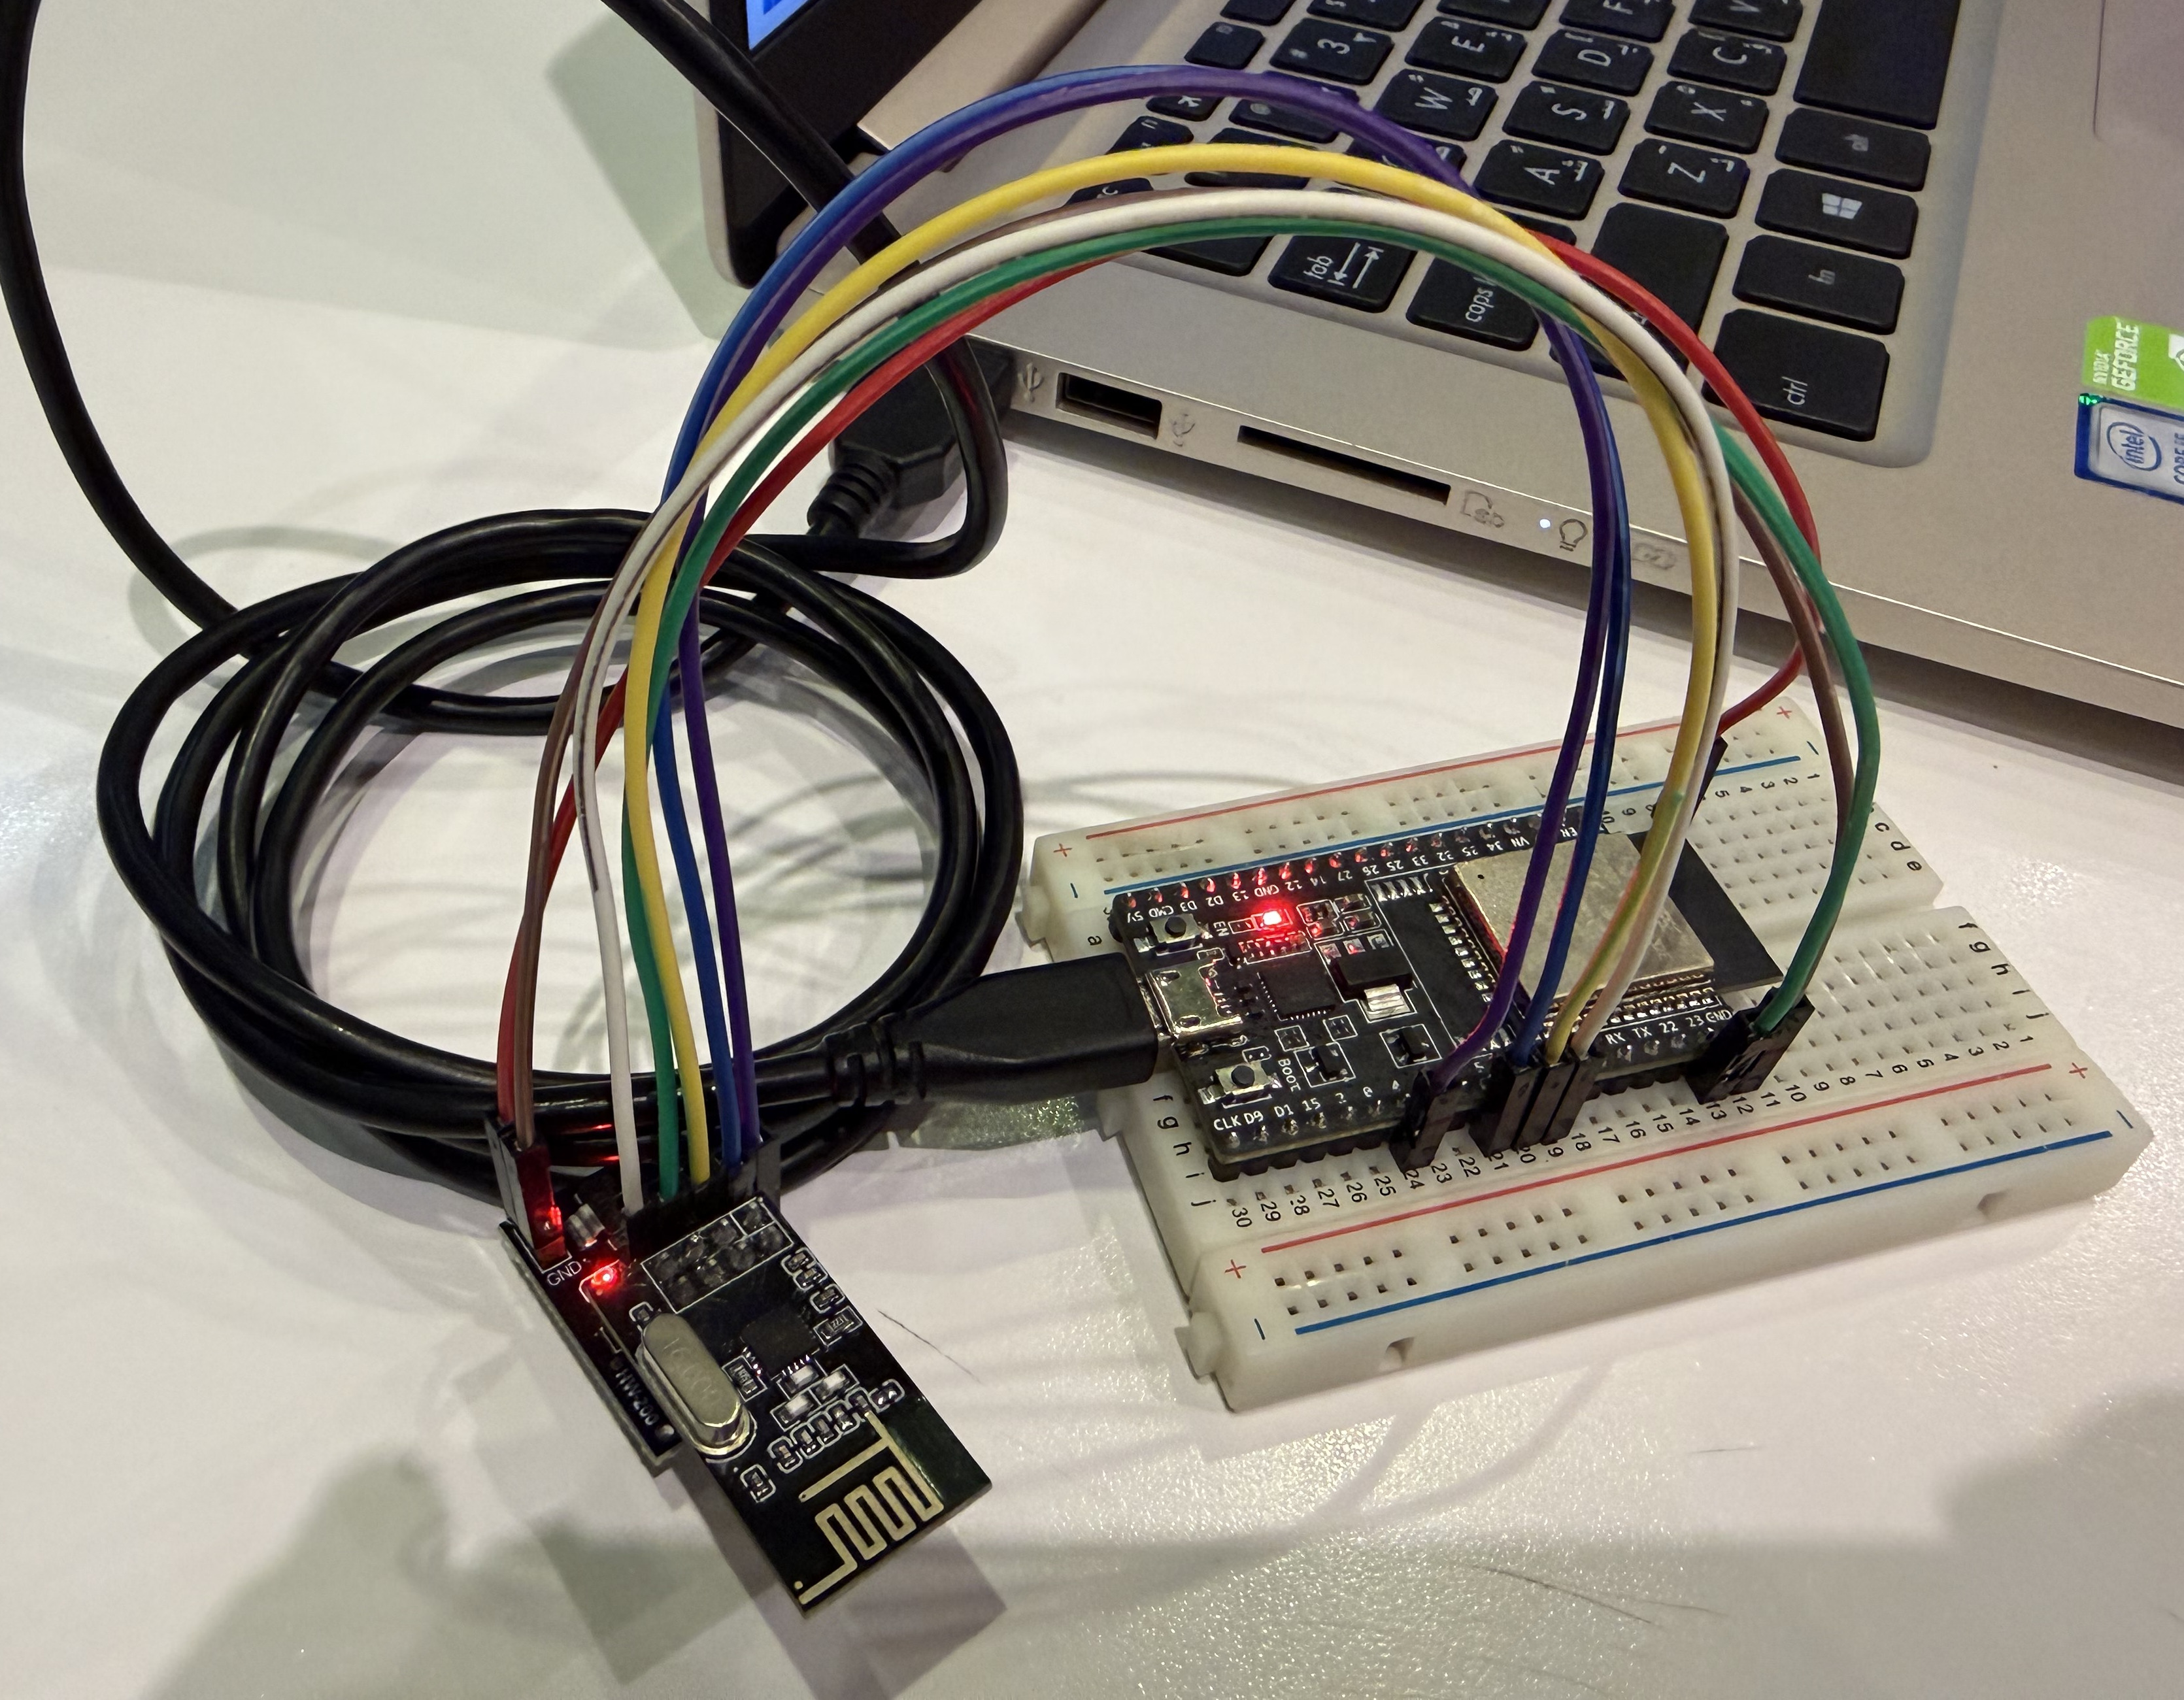
\includegraphics[width=0.55\textwidth, frame]{images/esp32 + nrf2401.jpeg}
\caption{ESP32-DevKitC V4 on a breadboard with the NRF24L01 module wired via jumper cables.}
\label{fig:esp32-nrf}
\end{figure}

The next step was to replace one of the ESP receivers with the STC board (Figure~\ref{fig:stc-board}). The NRF chip was inserted into the STC breakout board's dedicated socket, connected via bit-banged SPI on Port~1 (Table~\ref{tab:nrf-pins}), with 470\,$\Omega$ series resistors on the SPI lines. The NRF driver was adapted from an open-source 8051 implementation~\cite{cooledcoffee-nrf}, with the bit-banged SPI transferring each byte one bit at a time through the MOSI and MISO pins (Listing~\ref{lst:spi-rw}). The ESP continued transmitting its counter packets. Initial attempts showed no indication of reception on the STC side. Online suggestions pointed to a missing decoupling capacitor on the NRF supply; a 47\,$\mu$F capacitor was soldered in with a makeshift setup, but communication still failed. To rule out the ESP side, a second ESP and breakout board were used to confirm that the radio link worked between two ESPs. The problem was therefore isolated to the STC board.

\begin{figure}[ht]
\centering
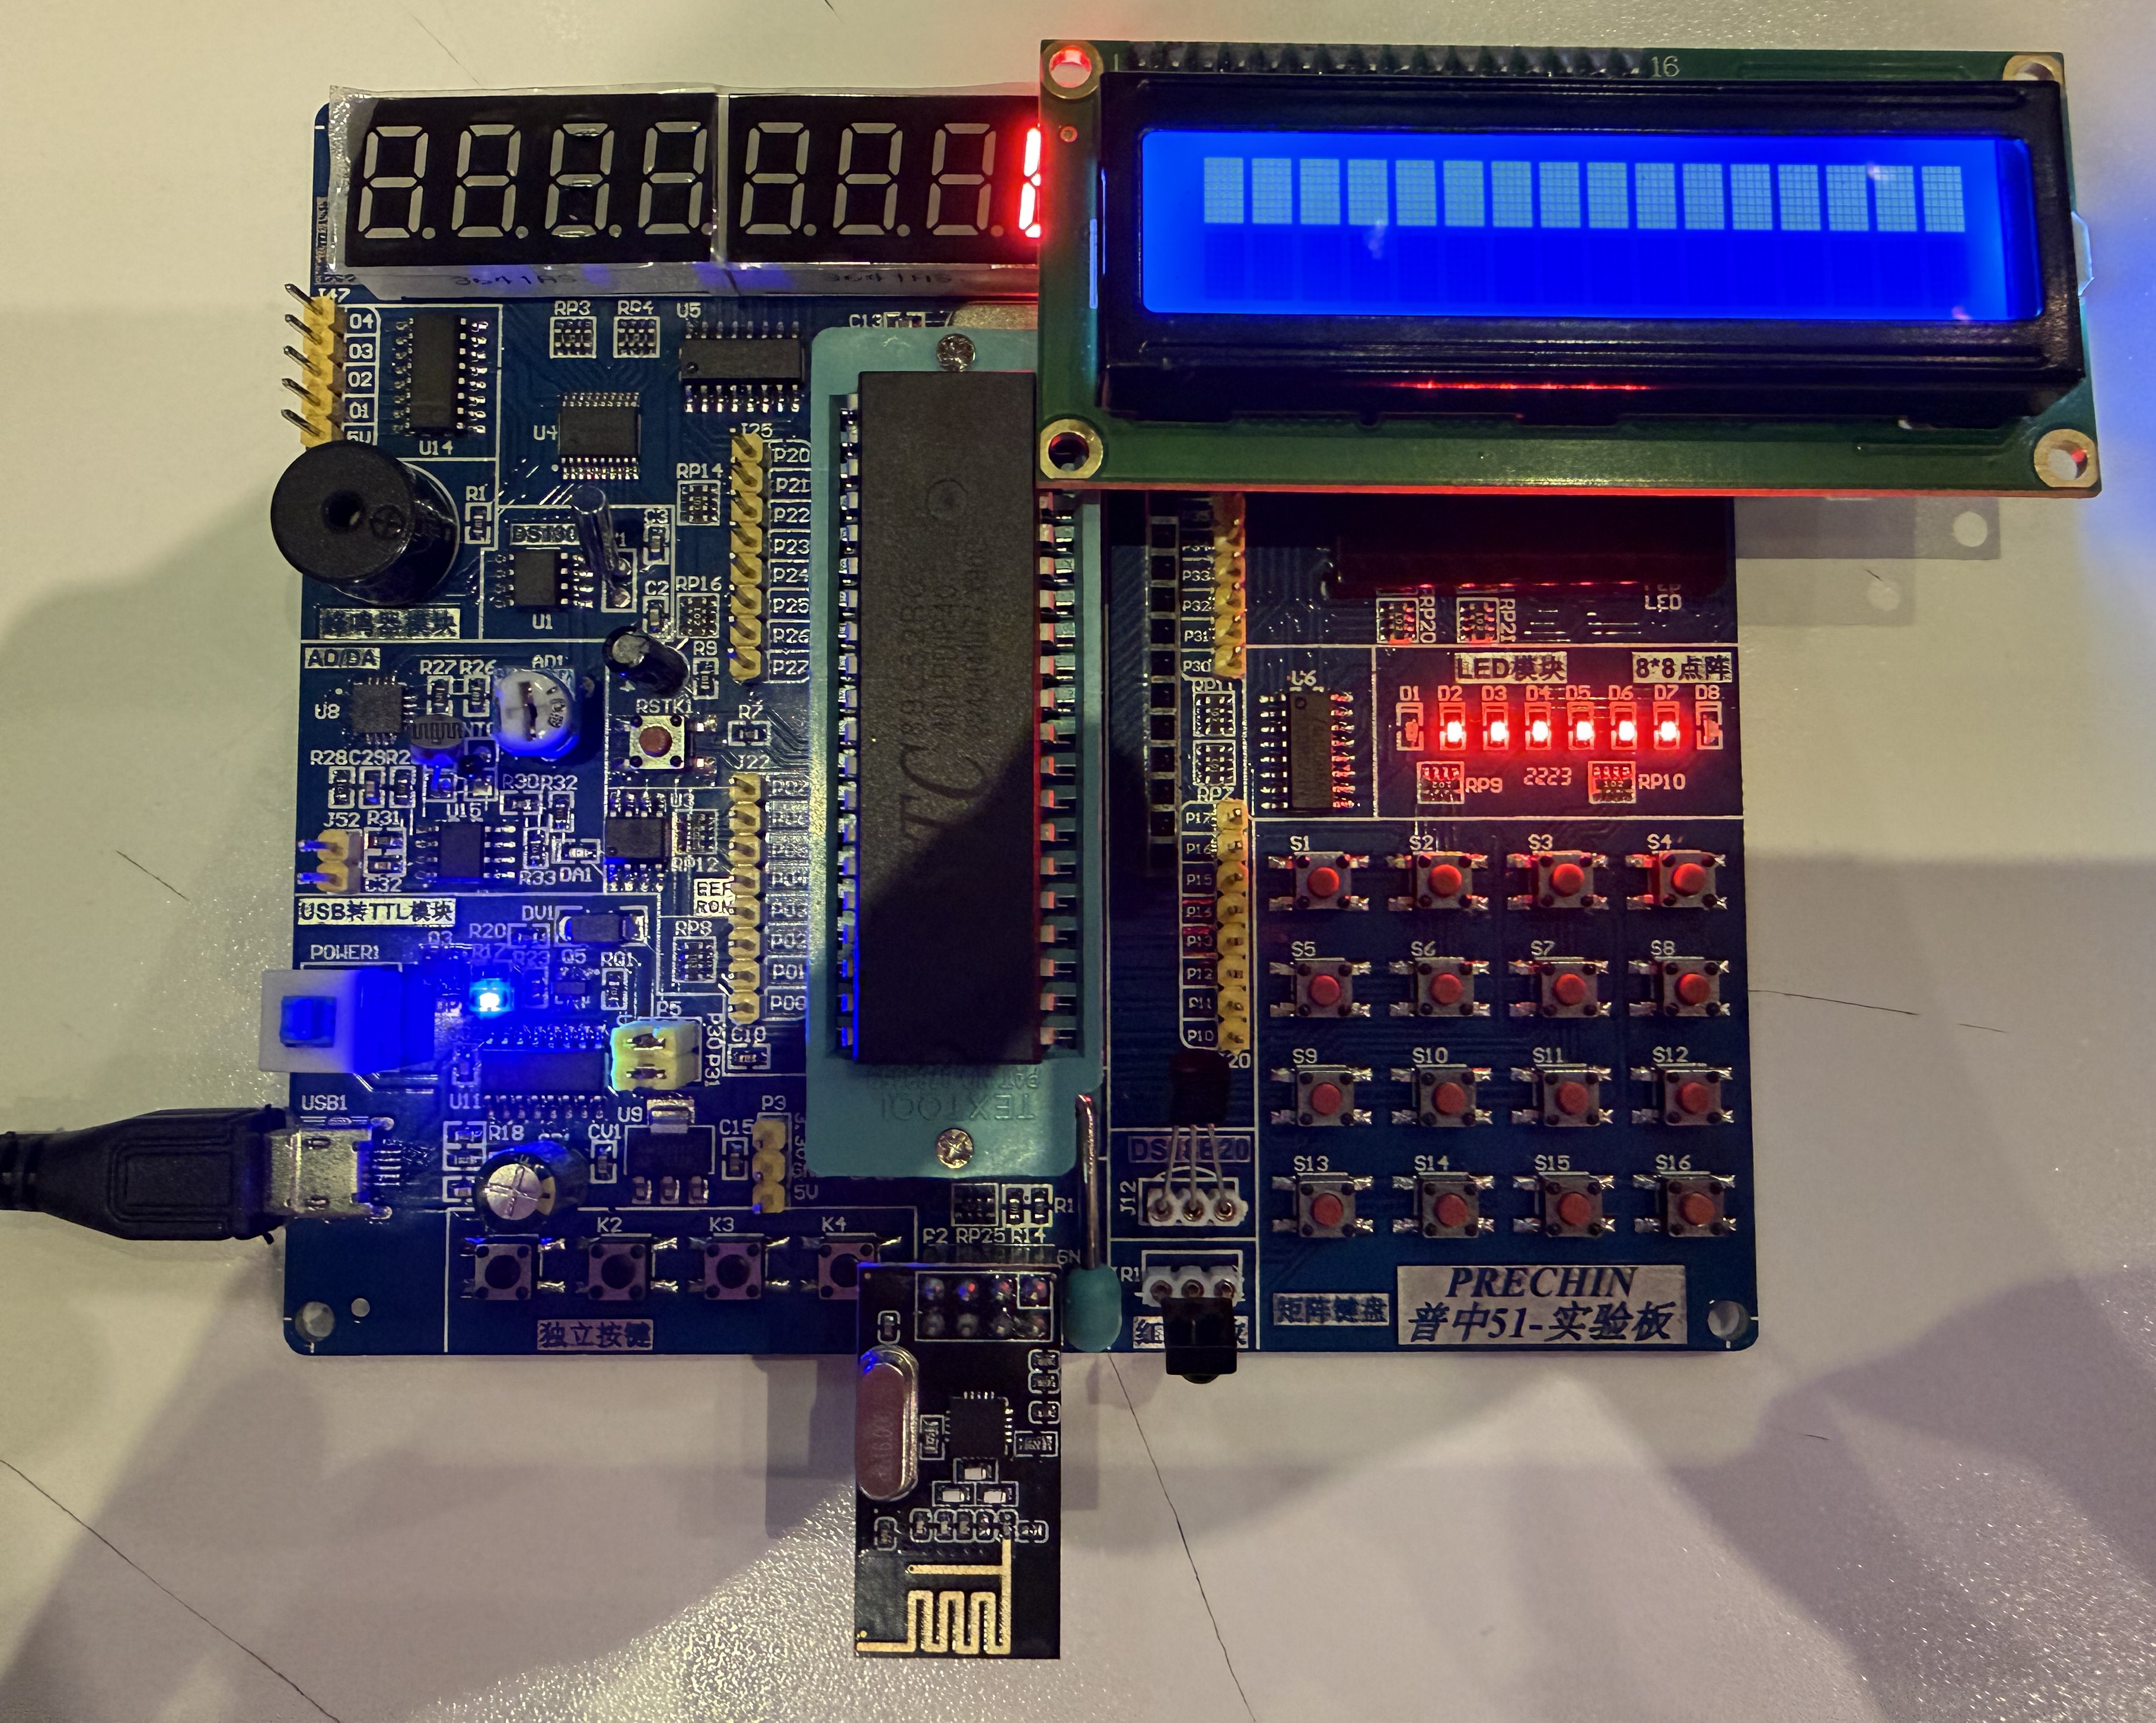
\includegraphics[width=0.55\textwidth, frame]{images/stc board + components.jpeg}
\caption{STC89C52RC breakout board with LCD1602 display and NRF24L01 module connected.}
\label{fig:stc-board}
\end{figure}

\begin{listing}[ht]
\inputminted[firstline=240, lastline=250, fontsize=\footnotesize, frame=single, linenos]{c}{../STC89C52/nrf24l01.h}
\caption{Bit-banged SPI byte transfer on the STC (\texttt{nrf24l01.h}).}
\label{lst:spi-rw}
\end{listing}

An LCD1602~\cite{hd44780} screen was connected to the STC board (8-bit data on P0, control lines on P2) to provide real-time debugging output. The firmware was modified to display NRF register values on the LCD after initialization. This revealed that certain register writes were being silently dropped. The channel register (\texttt{RF\_CH\,=\,108}) remained at its default value despite being written. Adding a 5\,ms delay before the configuration sequence allowed the first write to succeed. A second dropped register (auto-acknowledgement disable, \texttt{EN\_AA\,=\,0}) was fixed by inserting a dummy \texttt{STATUS} register read before the configuration writes, effectively waking the SPI bus. With both fixes in place, the STC began receiving packets from the ESP, and the 47\,$\mu$F capacitor was confirmed to be unnecessary. Bidirectional communication was then verified by temporarily converting the STC to a transmitter. The final initialization function incorporating all workarounds is shown in Listing~\ref{lst:nrf-config}.

\begin{listing}[ht]
\inputminted[firstline=188, lastline=206, fontsize=\footnotesize, frame=single, linenos]{c}{../STC89C52/nrf24l01.h}
\caption{NRF initialization with SPI timing workarounds (\texttt{nrf24l01.h}).}
\label{lst:nrf-config}
\end{listing}

With radio communication working, the pinging ESP firmware was replaced with a keyboard forwarder (\texttt{keyboard\_tx.cpp}). Instead of transmitting a counter, the ESP reads characters from its UART, batches them over a 20\,ms window, and packages them into a 32-byte payload: byte~0 holds the character count (1 to 30), bytes~1 to~30 hold the ASCII data, and byte~31 carries a sequence number. On the STC side, the receiver firmware interprets incoming characters and renders them on the LCD with cursor management, supporting backspace, enter (line break or clear), and Ctrl+L (full clear). A Python keyboard client captures keystrokes on the PC and forwards them to the ESP over serial. The system architecture is shown in Figure~\ref{fig:arch}.

As an initial reliability measure, each packet was transmitted five times with 1\,500\,$\mu$s spacing, and the receiver used sequence-number deduplication to discard repeated copies. This approach worked but was wasteful: it consumed five times the channel bandwidth regardless of whether the first copy arrived. Before replacing this scheme with a proper acknowledgement protocol, two improvements to the receiver were needed: more accurate polling and a way to send acknowledgements back to the transmitter.

\begin{figure}[ht]
\centering
\fbox{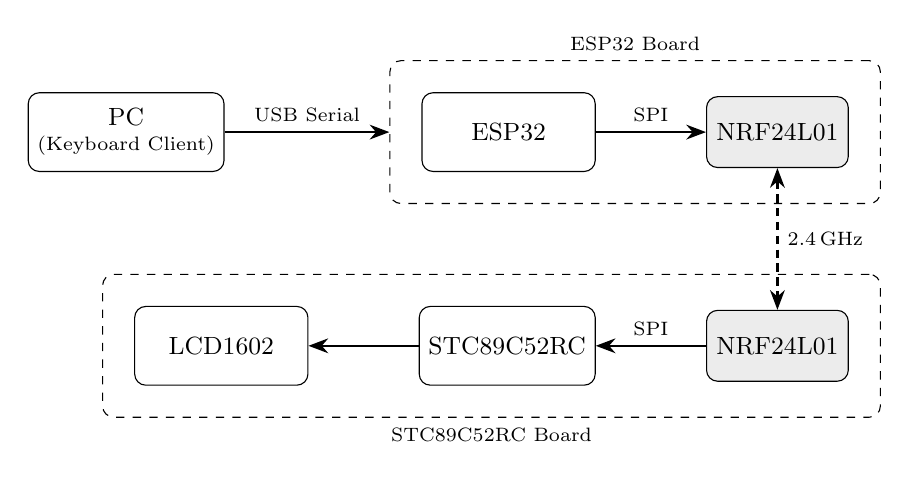
\begin{tikzpicture}[
    node distance=0.8cm and 1.4cm,
    box/.style={draw, rounded corners, minimum height=1cm, minimum width=2.2cm, align=center, font=\small},
    chip/.style={draw, rounded corners, minimum height=0.9cm, minimum width=1.8cm, align=center, font=\small, fill=gray!15},
    group/.style={draw, dashed, rounded corners, inner sep=0.4cm},
    arr/.style={-{Stealth[length=2.5mm]}, thick},
    lbl/.style={font=\scriptsize, midway},
]

% Top row: PC side
\node[box] (pc) {PC\\[-0.2em]{\scriptsize (Keyboard Client)}};
\node[box, right=2.5cm of pc] (esp) {ESP32};
\node[chip, right=of esp] (nrf1) {NRF24L01};

% Bottom row: STC side (right to left)
\node[chip, below=1.8cm of nrf1] (nrf2) {NRF24L01};
\node[box, left=of nrf2] (stc) {STC89C52RC};
\node[box, left=of stc] (lcd) {LCD1602};

% Group boxes
\node[group, fit=(esp)(nrf1), label={[font=\scriptsize]above:ESP32 Board}] (espgroup) {};
\node[group, fit=(stc)(nrf2)(lcd), label={[font=\scriptsize]below:STC89C52RC Board}] (stcgroup) {};

% Arrows
\draw[arr] (pc) -- node[lbl, above] {USB Serial} (espgroup.west |- esp);
\draw[arr] (esp) -- node[lbl, above] {SPI} (nrf1);
\draw[{Stealth[length=2.5mm]}-{Stealth[length=2.5mm]}, thick, densely dashed] (nrf1) -- node[lbl, right] {2.4\,GHz} (nrf2);
\draw[arr] (nrf2) -- node[lbl, above] {SPI} (stc);
\draw[arr] (stc) -- (lcd);

\end{tikzpicture}}
\caption{System architecture: PC keystrokes are forwarded through the ESP and NRF radio link to the STC, which displays them on the LCD. The dashed arrow is bidirectional: the STC sends acknowledgement packets back to the ESP over the same radio channel.}
\label{fig:arch}
\end{figure}

The initial receiver used a delay-based loop to poll the NRF for incoming packets, but the timing was imprecise: blocking operations in the main loop (LCD writes, UART prints) would stretch the polling interval unpredictably, risking overflow of the NRF's three-deep RX FIFO. To get accurate, consistent polling, the delay-based approach was replaced with a Timer~0 interrupt service routine (Listing~\ref{lst:timer0-isr}). The ISR fires every 5\,ms regardless of what the main loop is doing, checks the \texttt{STATUS} register for the \texttt{RX\_DR} flag, and drains any received packets from the FIFO into an 8-slot ring buffer in \texttt{xdata} memory. The main loop then consumes packets from the ring buffer at its own pace.

\begin{listing}[ht]
\inputminted[firstline=76, lastline=107, fontsize=\footnotesize, frame=single, linenos]{c}{../STC89C52/main.c}
\caption{Timer~0 ISR: polls the NRF every 5\,ms and drains received packets into a ring buffer (\texttt{main.c}).}
\label{lst:timer0-isr}
\end{listing}

To replace the 5$\times$ redundancy scheme with something more efficient, an application-level acknowledgement protocol was implemented. The NRF's built-in auto-acknowledgement feature was not used because it proved unreliable on clone modules. Instead, the protocol operates entirely in software. On the ESP side, after transmitting a packet, the radio switches to RX mode and waits up to 50\,ms for an ACK (Listing~\ref{lst:send-with-ack}). If no matching ACK arrives, the packet is retransmitted, up to 15 attempts. On the STC side, upon receiving a valid packet, the firmware immediately constructs a 32-byte ACK response (byte~0 set to \texttt{0xFF} as a marker, byte~31 carrying the matching sequence number) and transmits it back before performing any UART or LCD work (Listing~\ref{lst:send-ack}). This ACK-first ordering minimizes the response latency, keeping it well within the ESP's 50\,ms timeout window. Duplicate packets (same sequence number as the previous) are acknowledged but not processed, preventing repeated characters on the LCD. Listing~\ref{lst:rx-loop} shows the complete main-loop logic on the STC.

\begin{listing}[ht]
\inputminted[firstline=43, lastline=69, fontsize=\footnotesize, frame=single, linenos]{cpp}{../esp32_firmware/keyboard_tx.cpp}
\caption{ESP ACK-based transmission: send a packet, wait for acknowledgement, and retry on timeout (\texttt{keyboard\_tx.cpp}).}
\label{lst:send-with-ack}
\end{listing}

\begin{listing}[ht]
\inputminted[firstline=119, lastline=141, fontsize=\footnotesize, frame=single, linenos]{c}{../STC89C52/main.c}
\caption{STC ACK response: builds and sends an acknowledgement packet, then returns to RX mode (\texttt{main.c}).}
\label{lst:send-ack}
\end{listing}

\begin{listing}[ht]
\inputminted[firstline=228, lastline=261, fontsize=\footnotesize, frame=single, linenos]{c}{../STC89C52/main.c}
\caption{STC main loop: dequeues packets from the ring buffer, sends ACK immediately, then processes characters for the LCD (\texttt{main.c}).}
\label{lst:rx-loop}
\end{listing}

During reliability testing of the ACK protocol, delivery rates unexpectedly dropped to 0\% after code changes that should not have affected radio behavior. Diagnostic logging was added to the Timer~0 ISR to track interrupt counts, received packet counts, and the \texttt{STATUS} register value. The ISR was confirmed to be running correctly, and the \texttt{STATUS} register showed a clean state (\texttt{0x0E}), but no \texttt{RX\_DR} flags were ever set. Reading the Carrier Detect register (address \texttt{0x09}) returned \texttt{0x00} consistently, indicating that no RF signal was being detected at all. This pointed to a hardware fault rather than a software issue. Swapping the NRF module on the STC board with the one from the ESP board immediately restored communication. The faulty module's SPI interface was fully functional (register reads and writes returned correct values), but its RF front-end was not. Whether the receiver, transmitter, or both had failed was not investigated further, since the module swap resolved the issue and prior configurations had worked correctly with the replacement module.

With a working NRF module installed, a stress test was conducted to validate the ACK protocol under sustained load. The test sent 1000 characters at 0.1-second intervals using the keyboard client in automated mode. Because the ESP batches characters arriving within its 20\,ms window into a single packet, 1000 characters produce fewer than 1000 radio packets (typically 860 to 960, depending on timing). Table~\ref{tab:stress-runs} summarizes the results across six runs under varying conditions. All runs achieved 100\% delivery with zero failed packets out of approximately 5\,400 total. Table~\ref{tab:retry-dist} shows the per-packet retry distribution from a representative run. Over half of all packets (56.7\%) succeeded on the first attempt without any retries, and 87.6\% succeeded within two retries. Only 1.8\% of packets required five or more retries. The maximum observed retry count was 12, well within the 15-retry budget. Runs with LCD display operations added approximately 0.1 to 0.3 average retries per packet compared to runs without the LCD, consistent with the blocking LCD writes delaying the ACK response.

\begin{table}[ht]
\centering
\caption{Stress test results: 1000 characters per run at 0.1\,s intervals.}
\label{tab:stress-runs}
\begin{tabular}{cclccc}
\hline
Run & LCD & Packets & Delivery & Avg retries & Max retries \\
\hline
1 & No  & 956 & 100\% & 0.49 & 4  \\
2 & No  & 905 & 100\% & 0.70 & 5  \\
3 & Yes & 874 & 100\% & 0.81 & 7  \\
4 & Yes & 881 & 100\% & 0.83 & 8  \\
5 & Yes & 890 & 100\% & 0.83 & 7  \\
6 & Yes & 862 & 100\% & 0.91 & 12 \\
\hline
\end{tabular}
\end{table}

\begin{table}[ht]
\centering
\caption{Retry distribution from a representative 862-packet run (LCD enabled).}
\label{tab:retry-dist}
\begin{tabular}{ccc}
\hline
Retries & Count & Percentage \\
\hline
0  & 489 & 56.7\% \\
1  & 148 & 17.2\% \\
2  & 118 & 13.7\% \\
3  &  57 &  6.6\% \\
4  &  34 &  3.9\% \\
5  &   8 &  0.9\% \\
6  &   5 &  0.6\% \\
7  &   2 &  0.2\% \\
12 &   1 &  0.1\% \\
\hline
\end{tabular}
\end{table}

\begin{figure}[ht]
\centering
\includegraphics[width=0.75\textwidth, frame]{images/final.jpeg}
\caption{The complete system in operation: the keyboard client on the PC (top) sends typed text over serial to the ESP, which forwards it wirelessly to the STC board (bottom), displaying it on the LCD.}
\label{fig:final}
\end{figure}

\section{Discussion}

The main challenge was bringing up the NRF on the STC. Unlike the ESP, which has a mature RF24 library and hardware SPI, the STC relies on a bit-banged SPI implementation (Listing~\ref{lst:spi-rw}) that proved sensitive to initialization timing. Register writes issued too early after power-on were silently dropped, producing a radio configuration that looked correct in code but did not match what was actually loaded into the chip. Neither board has a hardware debugger; the only debugging options on the STC are the LCD screen, a canary LED, and UART serial output, while the ESP is limited to its built-in LED and serial output. Of these, serial output is the only channel accessible to Claude Code. Because the NRF provides no error feedback on failed writes, the only way to diagnose the problem was to read registers back and display them on the LCD or print them over UART. This trial-and-error debugging cycle consumed the majority of the development effort. The initial suspicion of a missing decoupling capacitor on the NRF supply turned out to be a red herring; the root cause was purely a software timing issue in the SPI initialization sequence.

A secondary challenge was the flashing workflow for the STC. The STC ISP protocol requires the MCU to be power-cycled to enter its bootloader, and the CH340G serial adapter's DTR pin, which automates this, had inverted polarity on the development board. This required patching the \texttt{stcgal} flashing tool at the source level. Additionally, after flashing, the NRF remains powered in whatever state it was last configured in, since only the MCU is reset. The initialization code must therefore force the radio into a known state (power-down, flush FIFOs, clear flags) before applying a fresh configuration, as shown in Listing~\ref{lst:nrf-config}.

Clone NRF modules introduced their own reliability issues. The 250\,kbps data rate, which should be supported by the chip, silently fails on clones and defaults back to 1\,Mbps. Auto-acknowledgement, another standard feature, proved unreliable. Both were worked around by fixing the data rate at 1\,Mbps and disabling auto-ack entirely. The initial workaround of transmitting each packet five times was later replaced by the application-level ACK protocol (Listings~\ref{lst:send-with-ack} and~\ref{lst:send-ack}), which retransmits only when needed and achieved 100\% delivery across all stress tests.

A separate challenge was diagnosing a faulty NRF module. Because the module's SPI interface worked correctly (all register reads and writes returned expected values), the failure appeared to be a software issue. The breakthrough came from reading the Carrier Detect register, which consistently returned zero, proving that no RF signal was reaching the receiver at all. This experience highlights a practical difficulty with clone NRF modules: partial hardware failures can mimic software bugs, and the chip provides limited diagnostic feedback beyond the Carrier Detect register.

The current system has several limitations that would need to be addressed for further extension. The LCD is limited to 16$\times$2 characters, providing no scrollback or history. The keyboard client is Windows-specific due to its use of \texttt{msvcrt} for keystroke capture. The breakout board's port multi-connection constraints leave very few free GPIO pins, making it difficult to add further peripherals without redesigning the board layout. The ACK protocol, while achieving 100\% delivery in testing, adds latency per packet due to the mode-switch overhead on the STC (temporarily switching from RX to TX to send the acknowledgement). For the keyboard use case this latency is imperceptible, but higher-throughput applications would benefit from the NRF's hardware auto-ack if reliable modules were used.

\section{Conclusion}

This project demonstrated that a resource-constrained 8051 microcontroller can be extended with wireless communication capabilities using low-cost NRF radio modules. By introducing the ESP as a USB-to-radio bridge, the NRF can communicate with the PC without requiring additional wiring on the STC's already constrained Prechin board. The resulting wireless keyboard allows a user to type on a PC and see characters appear on the STC's LCD display in real time over a 2.4\,GHz radio link. The main engineering effort lay in three areas: debugging the bit-banged SPI initialization on the STC side, where silent register drops required careful timing workarounds; diagnosing a faulty NRF module whose non-functional RF front-end mimicked a software bug; and implementing an application-level ACK protocol to replace the initial brute-force redundancy scheme. The final system achieved 100\% packet delivery across six stress tests totaling over 5\,000 packets, with an average of fewer than one retry per packet. The full source code, firmware, and build scripts are available at \url{https://github.com/marwan-humaid/wireless-8951}.

\begin{thebibliography}{9}

\bibitem{nrf24l01} Nordic Semiconductor, \textit{NRF24L01+ Single Chip 2.4\,GHz Transceiver Product Specification v1.0}, 2008.

\bibitem{stc89c52} STC Micro, \textit{STC89C52RC Datasheet}, STC Micro Technology Co.

\bibitem{rf24lib} TMRh20, \textit{RF24 Library for Arduino}, \url{https://github.com/nRF24/RF24}.

\bibitem{stcgal} Grigori Goronzy, \textit{stcgal: STC MCU ISP flash tool}, \url{https://github.com/grigorig/stcgal}.

\bibitem{hd44780} Hitachi, \textit{HD44780U (LCD-II) Dot Matrix Liquid Crystal Display Controller/Driver}, 1998.

\bibitem{esp32} Espressif Systems, \textit{ESP32-DevKitC V4 Getting Started Guide}, \url{https://docs.espressif.com/projects/esp-idf/en/latest/esp32/hw-reference/esp32/get-started-devkitc.html}.

\bibitem{cooledcoffee-nrf} CooledCoffee, \textit{NRF24L01 driver for 8051}, \url{https://github.com/CooledCoffee/nrf24l01}.

\end{thebibliography}

\newpage

\appendix

\section{Pinout Diagrams}

Figures~\ref{fig:pinout-nrf}, \ref{fig:pinout-stc}, and~\ref{fig:pinout-esp32} show the pinout diagrams for the three hardware modules used in this project.

\vspace{0.5cm}
\begin{figure}[ht]
\centering
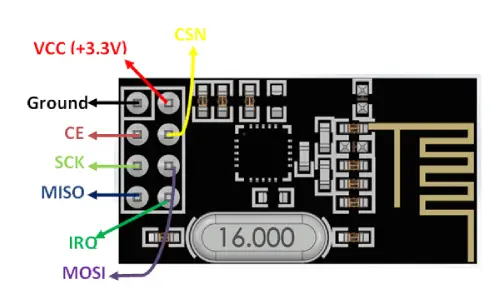
\includegraphics[width=0.28\textwidth, frame]{images/nrf2401 pinout.png}
\caption{NRF24L01 module pinout.}
\label{fig:pinout-nrf}
\end{figure}
\vspace{0.3cm}
\begin{figure}[ht]
\centering
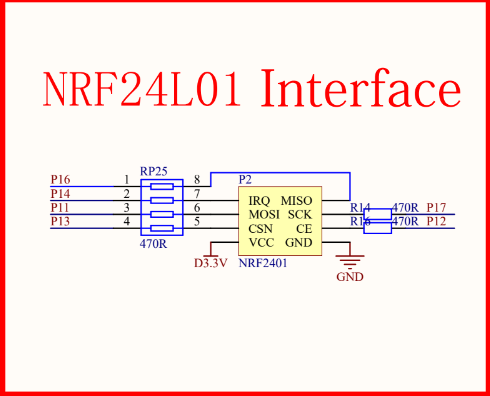
\includegraphics[width=0.28\textwidth, frame]{images/stc nrf2401 pinout.png}
\caption{STC89C52RC breakout board pinout.}
\label{fig:pinout-stc}
\end{figure}
\vspace{0.3cm}
\begin{figure}[ht]
\centering
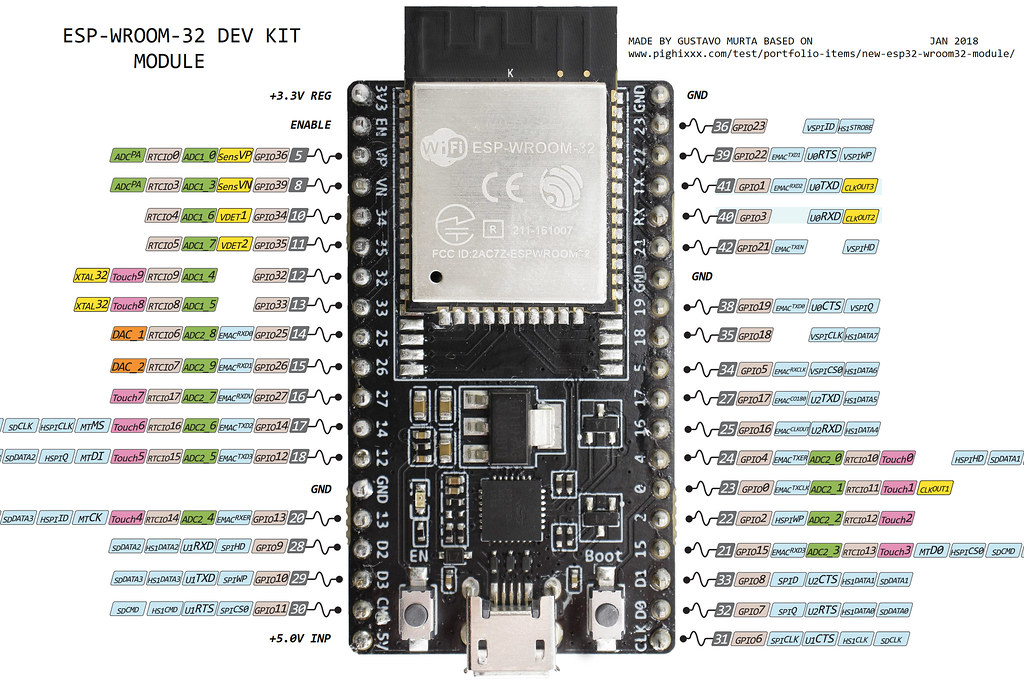
\includegraphics[width=0.65\textwidth, frame]{images/v4 pinout.jpg}
\caption{ESP32-DevKitC V4 pinout.}
\label{fig:pinout-esp32}
\end{figure}

\end{document}
